\documentclass[DIN, pagenumber=false, fontsize=11pt, parskip=half]{scrartcl}

\usepackage{amsmath}
\usepackage{amsfonts}
\usepackage{amssymb}
\usepackage{enumitem}
\usepackage[utf8]{inputenc} 
\usepackage[ngerman]{babel} 
\usepackage[T1]{fontenc} 
\usepackage{pgfplots}
\usepackage{xcolor}
\usepackage{listings}
\usepackage{float}
\usepackage{graphicx}
\usepackage{booktabs}
\usepackage{tkz-euclide}
\usepackage{svg}
\usepackage{trfsigns}
\usepackage{mathtools}

\DeclarePairedDelimiter\abs{\lvert}{\rvert}%
\DeclarePairedDelimiter\norm{\lVert}{\rVert}%

\definecolor{mygreen}{RGB}{28,172,0} % color values Red, Green, Blue
\definecolor{mylilas}{RGB}{170,55,241}

\tikzstyle{neuron}=[circle,fill=black!25,minimum size=30pt,inner sep=0pt]

\lstset{language=Matlab,%
    %basicstyle=\color{red},
    breaklines=true,%
    morekeywords={matlab2tikz},
    keywordstyle=\color{blue},%
    morekeywords=[2]{1}, keywordstyle=[2]{\color{black}},
    identifierstyle=\color{black},%
    stringstyle=\color{mylilas},
    commentstyle=\color{mygreen},%
    showstringspaces=false,%without this there will be a symbol in the places where there is a space
    numbers=left,%
    numberstyle={\tiny \color{black}},% size of the numbers
    numbersep=9pt, % this defines how far the numbers are from the text
    emph=[1]{for,end,break},emphstyle=[1]\color{red}, %some words to emphasise
    %emph=[2]{word1,word2}, emphstyle=[2]{style},    
}

\title{Einführung in die Neuroinformatik}
\author{Tim Luchterhand, Paul Nykiel (Gruppe P)}

\begin{document}
    \maketitle
    \section{Kohonen's selbstorganisierende Karte}
    \subsection{}
    \begin{enumerate}[label=(\alph*)]
        \item $ $
            \begin{figure}[H]
                \centering
                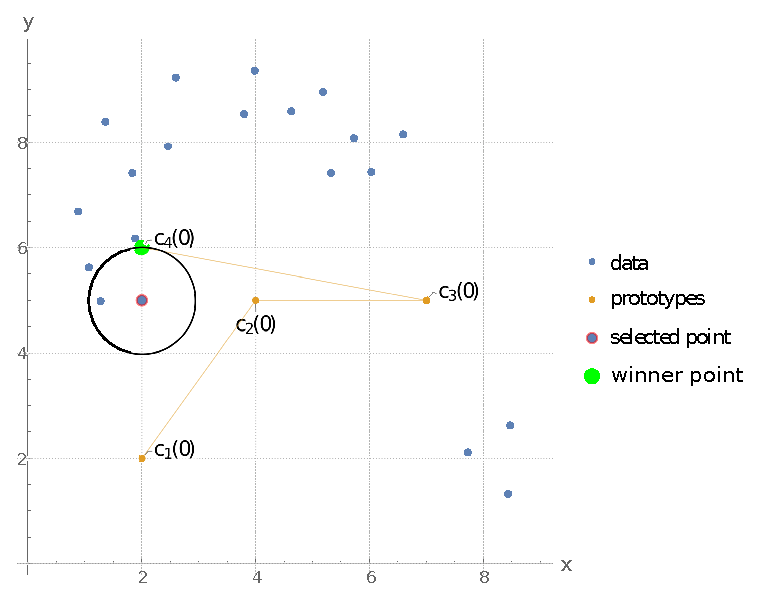
\includegraphics[width=.9\textwidth]{winner}
                \caption{Graphische Bestimmung des Gewinners}
            \end{figure}
        \item
            \begin{eqnarray*}
                c_j (t + 1) &=& c_j(t) + \eta(t) \cdot  \mathcal{N}_t (g_j , g_{j^{*}}) \cdot (x - c_j(t)) \\
                \eta(0) &=& \eta_\text{start} = 1 \\
                c_1 (1) &=& \begin{pmatrix} 2 \\ 2 \end{pmatrix} + \eta(0) \cdot \mathcal{N}_0 (1, 4) \cdot \left(\begin{pmatrix} 2 \\ 5\end{pmatrix} - \begin{pmatrix} 2 \\ 2 \end{pmatrix}\right) \\
                    &=& \begin{pmatrix} 2 \\ 2.0003 \end{pmatrix} \\
                c_2 (1) &=& \begin{pmatrix} 4 \\ 5 \end{pmatrix} + \eta(0) \cdot \mathcal{N}_0 (2, 4) \cdot \left(\begin{pmatrix} 2 \\ 5\end{pmatrix} - \begin{pmatrix} 4 \\ 5 \end{pmatrix}\right) \\
                    &=& \begin{pmatrix} 3.9662 \\ 5 \end{pmatrix} \\
                c_3 (1) &=& \begin{pmatrix} 7 \\ 5 \end{pmatrix} + \eta(0) \cdot \mathcal{N}_0 (3, 4) \cdot \left(\begin{pmatrix} 2 \\ 5\end{pmatrix} - \begin{pmatrix} 7 \\ 5 \end{pmatrix}\right) \\
                    &=& \begin{pmatrix} 5.198 \\ 5 \end{pmatrix} \\
                c_4 (1) &=& \begin{pmatrix} 2 \\ 6 \end{pmatrix} + \eta(0) \cdot \mathcal{N}_0 (4, 4) \cdot \left(\begin{pmatrix} 2 \\ 5\end{pmatrix} - \begin{pmatrix} 2 \\ 6 \end{pmatrix}\right) \\
                    &=& \begin{pmatrix} 2 \\ 5 \end{pmatrix} \\
            \end{eqnarray*}
    \end{enumerate}

    \subsection{}
    Die Nachbarschaftserhaltung ist eine allgemeine Eigenschaft des Algorithmus, da letzendlich versucht wird, ein Gitter wie aus $\{g_1, \ldots, g_n\}$ 
    geschickt in die Datenpunkte zu legen.
\end{document}
